\documentclass[12pt]{beamer}
\usetheme[whale]{Hannover}
\usepackage[utf8]{inputenc}
\usepackage{subfig}
\usepackage{graphicx}
\title{Web-basierte Registrierkasse}
\author{Lukas Gritsch Benjamin Cilga}

\begin{document}


\begin{frame}[plain]
\maketitle
\small
\end{frame}

\begin{frame}
	\tableofcontents
\end{frame}


\section{Praktische Ausarbeitung und Programmierung}

\begin{frame}
\frametitle{Übersicht}
\Large Funktionsweise
\begin{figure}[h]
	\centering
	\subfloat[MVC-Pattern]{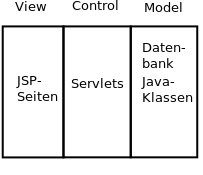
\includegraphics[scale=0.6]{Bilder/MVC.png}} \hfill
	\subfloat[Modell]{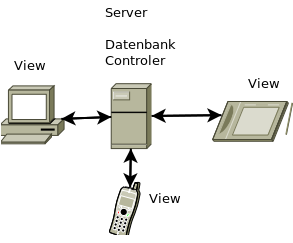
\includegraphics[scale=0.5]{Bilder/Modell.png}}
	
\end{figure}
\end{frame}

\subsection{Einarbeitungsphase}

\begin{frame}
\frametitle{Einarbeitungsphase}
\begin{Large}
Einlesen in die Vorgängerarbeit\\ \vspace{0.2 cm}
Laravel oder Servlets und JSP ? \vspace{1 cm}
\end{Large}

\begin{tabular}{l|l}
\textbf{Laravel:} & \textbf{Servlets und JSP}\\ \hline
PHP Framework & Java und JSP Dateien\\
Vereinfachter Syntax & Java und HTML Syntax\\
Eigenes Datenbankdesign & Keine Designvorgabe
\end{tabular}

\end{frame}

\subsection{Umsetzungsphase}
\begin{frame}
\frametitle{Umsetzungsphase}
\begin{itemize}
	\item[-] Programmierung ---- Problem (Schwierigkeiten)
\end{itemize}
\end{frame}


\subsection{Testphase}
\begin{frame}
\frametitle{Testphase}
	\begin{itemize}
		\item[-] Verwendung des Rasperry Pi --(Was ist ein Rassperry Pi -- Bilder --- verwendung als)
	\end{itemize}
\end{frame}

\section{Wirtschaftliche Vorarbeit}
\subsection{Marktforschung}
\begin{frame}
\frametitle{Fragebogen}
\end{frame}

\subsection{Umfragen}

\begin{frame}

\end{frame}

\subsection{Stinken}
\begin{frame}

\end{frame}

\begin{figure}
	\listoffigures
\end{figure}

\end{document}
